\chapter{РЕШЕНИЕ ЗАДАЧИ КЛАССИФИКАЦИИ}

В данной главе будут предложены несколько алгоритмов классификации вредоносных файлов, позволяющих с приемлемым качеством определять метку объектов, подготовленных нами ранее.
Действия в этой главе являются заключительными для создания классификатора. Мы будем использовать результат работы предыдущих глав, где мы создали необходимую выборку файлов, включающую в себя как вредоносные файлы, так и файлы, не причиняющие никакого вреда, а также собрали информацию о работе процесса “Microsoft Word”, специальным образом подготавливая каждый файл из выборки для запуска.

На практике очень часто методы машинного обучения тесно связаны с рассматриваемыми объектами и признаками, которые могут быть извлечены из них. Поэтому каждый предложенный нами алгоритм окажется отдельным подходом извлечения формального набора признаков для каждого исследуемого объекта. В зависимости от типа получившихся факторов мы будем использовать подходящий метод машинного обучения.

\section{Процесс как последовательность действий}

Для построения первой модели, мы рассмотрим процесс исполнения программы Microsoft Word, во время открытия каждого файла, как последовательность простых операций. В качестве операции будут выступать вызовы функций WinAPI, регистрируемые утилитой PROCMON, например такие как открытие файла, запись в файл или загрузка динамической библиотеки.

Во время создания того или иного набора признаков, принято обосновывать почему именно такой подход имеет право на жизнь. В нашем случае мы будем опираться на следующее предположение: последовательность действий, совершаемых вредосными файлами отличаются от нормального исполнения обычных пользовательских файлов. 

Имея на руках последовательность действий мы будем использовать технику, часто применяемую для построения различных языковых моделей натуральных языков. Только в отличии от традиционного использования таких методов, отдельным элементом языка у нас будет не слово на английском или русском языках, а операция, совершаемая запущенной программой. Каждый процесс в таком случае можно представить как документ, содержащий одно длинное предложение со словами из заданого множества.

Первый шаг необходимый для построения данной модели это перевод сырых данных, собранных с помощью утилиты PROCMON для каждого файла, в вектор слов. В нашем случае слово будет принадлежать конечному множеству операций, которые поддерживает PROCMON для перехвата, при этом мы будем рассматривать только подмножество операций непосредственно совершаемых Microsoft Word’ом и перехваченных во время исполнения.

\bgroup
\def\arraystretch{1.5}%  1 is the default, change whatever you need
\begin{table}[ht]
\caption{Пример операций и их отображений}
\label{tab_weight}
\centering
    \begin{tabular}{|c|c|}
    \hline \rowcolor{lightgray!50} Операция & Сокращённое обозначение \\
    \hline Process Start &  0 \\
    \hline Thread Create &  1 \\
    \hline QueryNameInformationFile &  2 \\
    \hline Load Image &  3 \\
    \hline CreateFile &  4 \\
    \hline
    \end{tabular}
\end{table}
\egroup

Для дальнейшей работы с этими операциями нам будет удобно отобразить их в короткие численные представления. Используя всё выше сказанное мы можем рассматривать элементы выборки как большие предложения, состоящие из чисел.

\newpage
\bgroup
\def\arraystretch{1.5}%  1 is the default, change whatever you need
\begin{table}[ht]
\caption{Первые 10 операций, совершаемые запущенной программой, и их отображения}
\label{tab_weight}
\centering
    \begin{tabular}{|c|c|}
    \hline \rowcolor{lightgray!50} Операция & Отображение \\
    \hline Process Start &  0 \\
    \hline Thread Create &  1 \\
    \hline QueryNameInformationFile &  2 \\
    \hline Load Image &  3 \\
    \hline Load Image &  3 \\
    \hline CreateFile &  4 \\
    \hline QueryDeviceInformationVolume &  5 \\
    \hline QueryOpen &  6 \\
    \hline Load Image &  3 \\
    \hline CreateFile &  4 \\
    \hline
    \end{tabular}
\end{table}
\egroup

Например, если допустить что Таблица 4.2 содержит результат работы программы Microsoft Word от начала до конца, то объект, сгенерировавший данные операции, будет иметь вид: \textbf{“0 1 2 3 3 4 5 6 3 4”}.

Один из случаев, которые мы сможем определить такой моделью, является вызов некоторой аномальной функции, совершающей потенциально зловредные действия. Тогда слово, соответствующее отображению этой функции в число, не будет принадлежать никакому предложению, составленному по безвредным объектам. В таком сценарии мы можем использовать распределение частот по каждому слову, состоящему из цифр, для принятия решения. Однако, в некоторых случаях для нас может представлять опасность не только отдельный вызов функций, а некоторая последовательность вызовов безобидных подпрограм. Например, последовательность функций “CreateFile”, “ReadFile”, “WriteFile” может служить сигналом о создании копии вируса в системе. Чтобы учесть такие ситуации, мы будем использовать распределение N-грамм как обобщение частот отдельных слов. 

N-граммы для N равного 1 представляют из себя частоты каждого слова документа в отдельности. Для $N$ равного 2 это распределение пар слов и т.д. Например, рассмотрим такое распределение для объекта из Таблицы 4.2, где $N$ принимает значения из множества $\{1,2\}$.

\bgroup
\def\arraystretch{1.5}%  1 is the default, change whatever you need
\begin{table}[ht]
\caption{Разложение объекта из Таблицы 4.2 на $N$-граммы для $N \in \{1, 2\}$}
\label{tab_weight}
\centering
    \begin{tabular}{|c|c|c|c|c|c|c|c|c|c|c|c|c|c|c|c|}
    \hline \rowcolor{lightgray!50} Тип N-граммы & 0 & 1 & 2 & 3 & 4 & 5 & 6 & 0 1 & 1 2 & 2 3 & 3 3 & 3 4 & 4 5 & 5 6 & 6 3 \\
    \hline Частота & 1 & 1 & 1 & 3 & 2 & 1 & 1 & 1 & 1 & 1 & 1 & 2 & 1 & 1 & 1 \\
    \hline
    \end{tabular}
\end{table}
\egroup

Количество различных N-грамм, конечно, зависит от самого значения числа N, поэтому его нужно выбирать из соображений баланса между длиной потенциально вредной последовательности и размером конечной матрицы объект-признак. В нашем случае для создания рабочего метода мы будем использовать N равное 3 ( Рассмотреть набор экспериментов для N от 1 до 3 и указать что разницы большой нет. Обосновать почему именно 3). Таким способом мы переведём каждый объект в вектор частот, получив в итоге матрицу объект-признак. Как и в примере с объектом из таблицы 1, в качестве признака будет частота определённой N-граммы встретившейся в каждом объекте из обучающей выборки.

Это и дальнейшие преобразования будут производиться с помощью библиотеки scikit-learn для языка Python. ( Подробней про эти библиотеки и про язык ).

\bgroup
\def\arraystretch{1.5}%  1 is the default, change whatever you need
\begin{table}[ht]
\caption{Фрагмент матрицы объект-признак для двух хороших $\{G_0, G_1\}$ и двух плохих $\{B_0, B_1\}$ файлов.}
\label{tab_weight}
\centering
    \begin{tabular}{|c|c|c|c|c|c|c|c|c|c|c|c|c|c|c|c|c|c|c|c|c|}
    \hline & \multicolumn{20}{c|}{Различные виды $N$-грамм} \\
    \hline $G_0$ & 38 & 5 & 91 & 17 & 10 & 2 & 4 & 1 & 1 & 1 & 1 & 1 & 2 & 0 & 0 & 0 & 0 & 0 & 0 & 0 \\
 	\hline $G_1$ & 49 & 5 & 16 & 17 & 10 & 2 & 5 & 1 & 1 & 1 & 1 & 1 & 2 & 2 & 4 & 0 & 0 & 0 & 0 & 0 \\
 	\hline $B_0$ & 285 & 9 & 78 & 85 & 79 & 3 & 15 & 5 & 1 & 1 & 3 & 3 & 0 & 7 & 12 & 1 & 3 & 1 & 5 & 1 \\
 	\hline $B_1$ & 288 & 8 & 81 & 85 & 79 & 2 & 8 & 1 & 1 & 1 & 3 & 3 & 0 & 4 & 12 & 1 & 0 & 0 & 2 & 0 \\
	\hline
    \end{tabular}
\end{table}
\egroup

Имея на руках данную матрицу, мы можем воспользоваться ранее описаной линейной моделью. После обучения метода и проверки качества классификации с помощью подсчёта ошибок техникой LOO, мы заметим что метод со 100 процентным качеством определяет вредоносные файлы. То есть составленная нами выборка линейно разделима по какому-то набору признаков. Мы можем найти примеры таких признаков.

\bgroup
\def\arraystretch{1.5}%  1 is the default, change whatever you need
\begin{table}[ht]
\caption{Фрагмент матрицы объект-признак для двух хороших $\{G_0, G_1\}$ и двух плохих $\{B_0, B_1\}$ файлов.}
\label{tab_weight}
\centering
    \begin{tabular}{|c|c|c|}
    \hline Вид файла & QueryAllInformationFile, FileSystemControl \\
    \hline $G_0$ & 0 \\
 	\hline $G_1$ & 0 \\
 	\hline $B_0$ & 2 \\
 	\hline $B_1$ & 2 \\
	\hline
    \end{tabular}
\end{table}
\egroup

Нашу выборку можно разделить по последовательностям действий представленным в Таблице 4.5. Для нас это означает что существует последовательность операций, совершаемых только вредоносными объектами. Не смотря на идеальную точность, данный результат считается недостаточно полным без дальнешего анализа происхождения данных операций, но подробный разбор работы Microsoft Word в случаях эксплуатаций различных уязвимостей является достаточно крупной задачей, достойной рассмотрения в отдельной работе. Мы же ограничимся получившимся результатом, как первичной грубой оценкой при первичном анализе зловредных объектов. ( Показать в исходных данных найденный паттерн. Подробней написать как модель    работает. )
Следующий метод основан на более сложном подходе, требующий объединения нескольких алгоритмов машинного обучения.

\section{Процесс как набор графиков}

В предыдущем параграфе был рассмотрен подход, основанный на разбиении выполнения процесса на простые операции с последующим анализом сгенерированных последовательностей операций.

Ранее нами было описан общий план проникновения и исполнения зловредного кода через эксплуатацию уязвимостей в сложных форматах файлов. Одним из этапов заражения является подготовка атакуемой программы для запуска шелл-кода. Часто в этот момент программа начинает вести себя необычно: зависать, работать медленней или аварийно завершаться. Чтобы отлавливать подобные ситуации автоматически, нам необходимо ввести набор формальных признаков, способных различать такие ситуации. Однако мы не можем подстраиваться под определённый вид поведения, например, завершение программы, потому что новый вирус, способный избегать появление такого демаскирующего признака, ускользнёт из нашего исследования.

В качестве обобщённого набора признаков, не привязанных к определённому виду визуального проявления, мы будем рассматривать время исполнения каждой операции. Время как признак является довольно чувствительными показателем работы процесса, если процесс будет вести себя необычно, то это прямо скажется на численных показателях времени. Исходя из таких рассуждений, был разработан новый метод извлечения формальных признаков работы из запущенной программы, основанный на представлении работы процесса в виде двумерного графика, где по оси X мы будем отображать номер операции, а по оси Y затраченное время на выполнение этой операции. 

То есть теперь в качестве признака выступает график, а не одно число, как в случае с частотой N-грамм. Это более богатое семейство, в отличии от N-грамм составленных по последовательностям из простых операций.

\newpage
\begin{figure}[ht]
	\centering
    \begin{subfigure}[b]{1\textwidth}
    \centering
        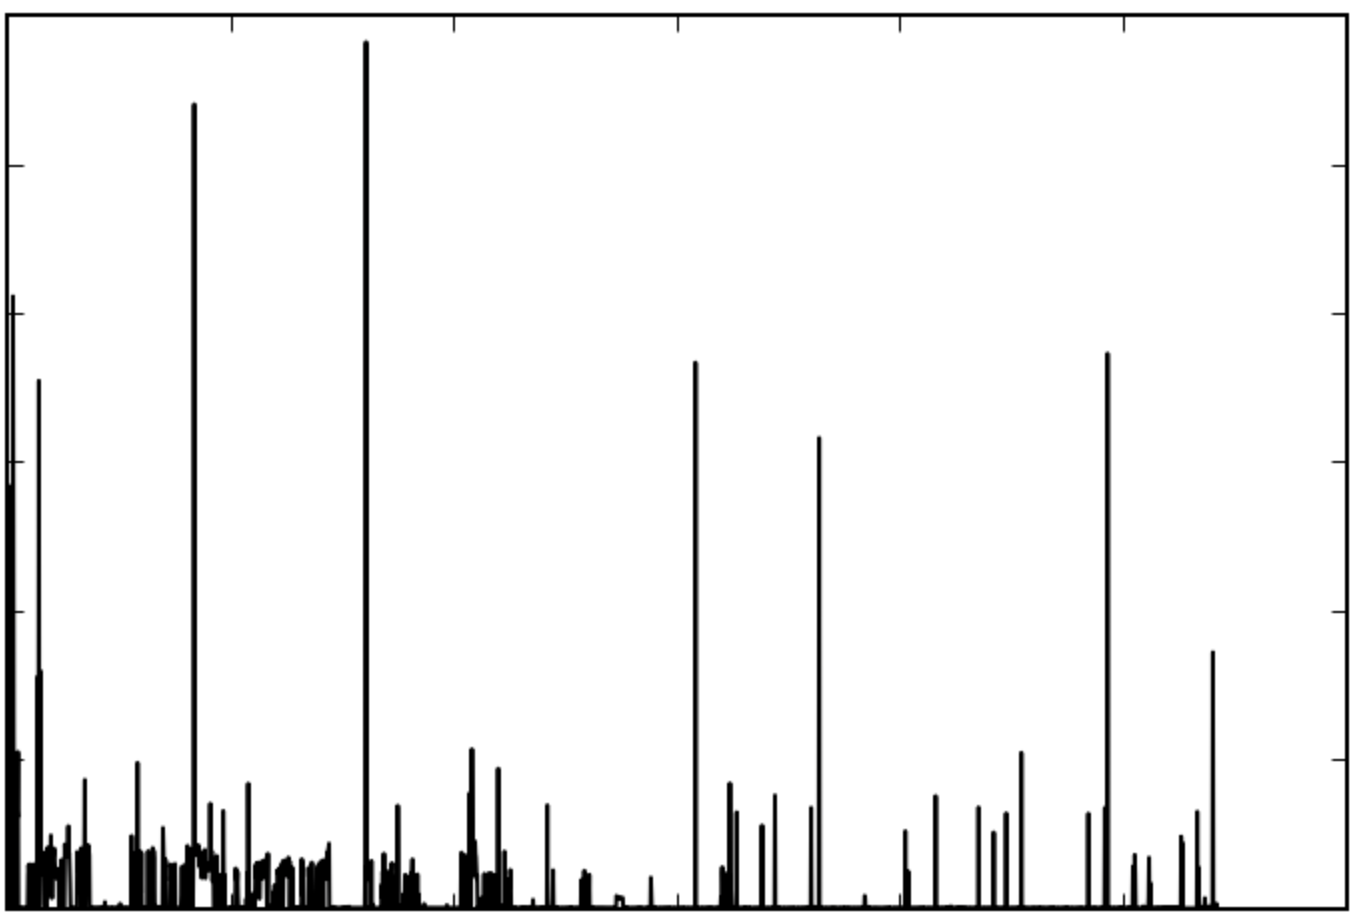
\includegraphics[scale=0.5]{pasted-image-29.png}
    \end{subfigure}
 
    \caption{График длительностей выполнения всех операций в течении работы одного из процессов Microsoft Word}
    \label{fig_parsetree}
\end{figure}

В графике, изображённом на Рисунке 4.1, по оси X были отображены операции всех типов в порядке их перехвата утилитой PROCMON. При работе больших программ вроде Microsoft Word многие операции производятся асинхронно, это означает что порядок некоторых групп операций неопределён. Как способ борьбы с этой проблемой мы можем разделить большой график, включающий все операций, на множество графиков, отображающих каждый тип операции в отдельности. Работа с множеством графиков также позволяет использовать некоторое подмножество операции, дающих наибольший прирост к качеству классификации. Подробности реализации такого отбора, будут рассмотрены в дальнейших параграфах.

\begin{figure}[ht]
	\centering
    \begin{subfigure}[b]{0.40\textwidth}
    \centering
        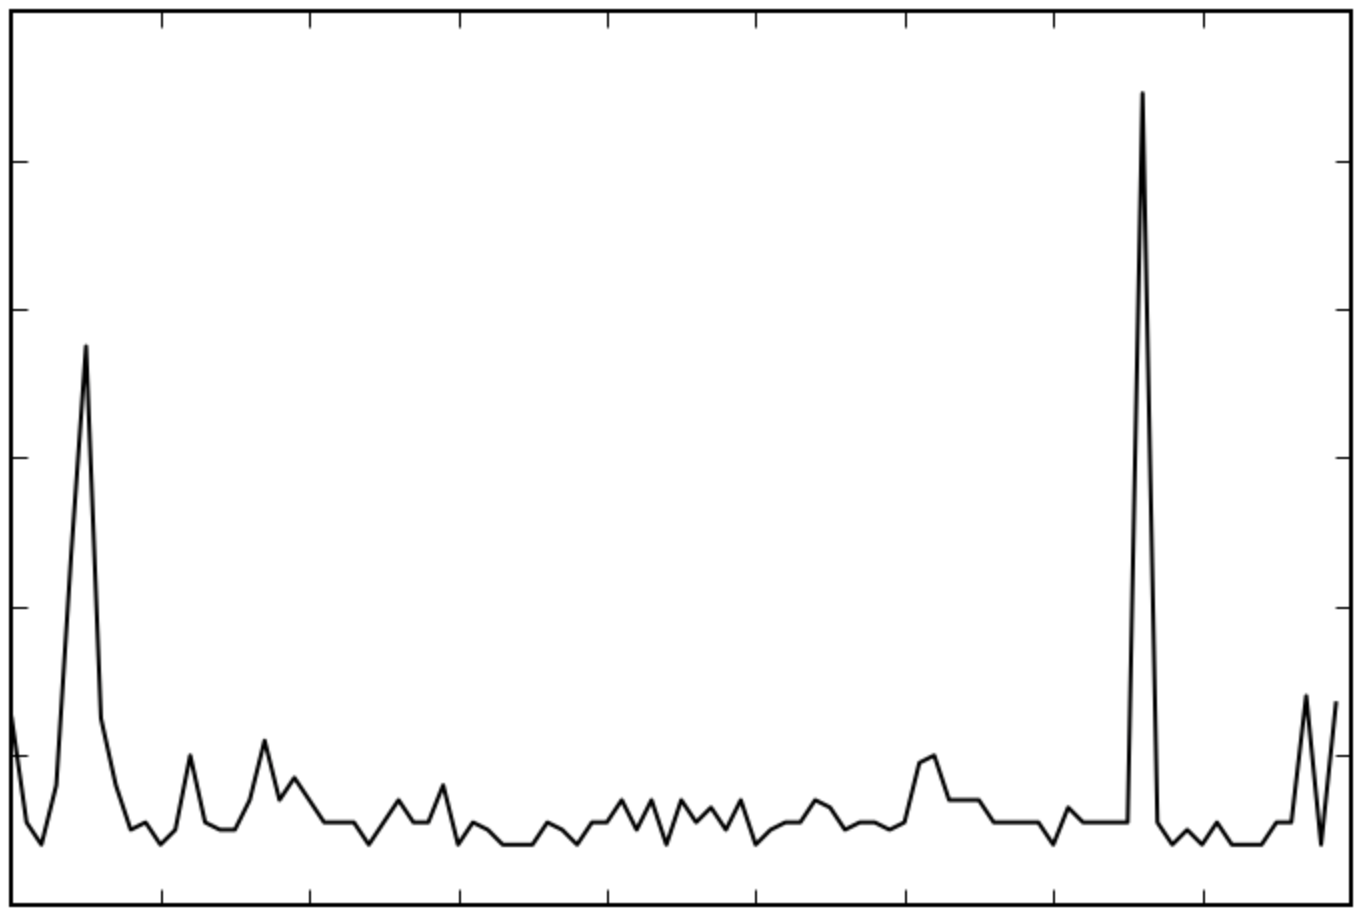
\includegraphics[scale=0.25]{pasted-image-31.png}
        \caption{}
    \end{subfigure}
 	\begin{subfigure}[b]{0.40\textwidth}
    \centering
        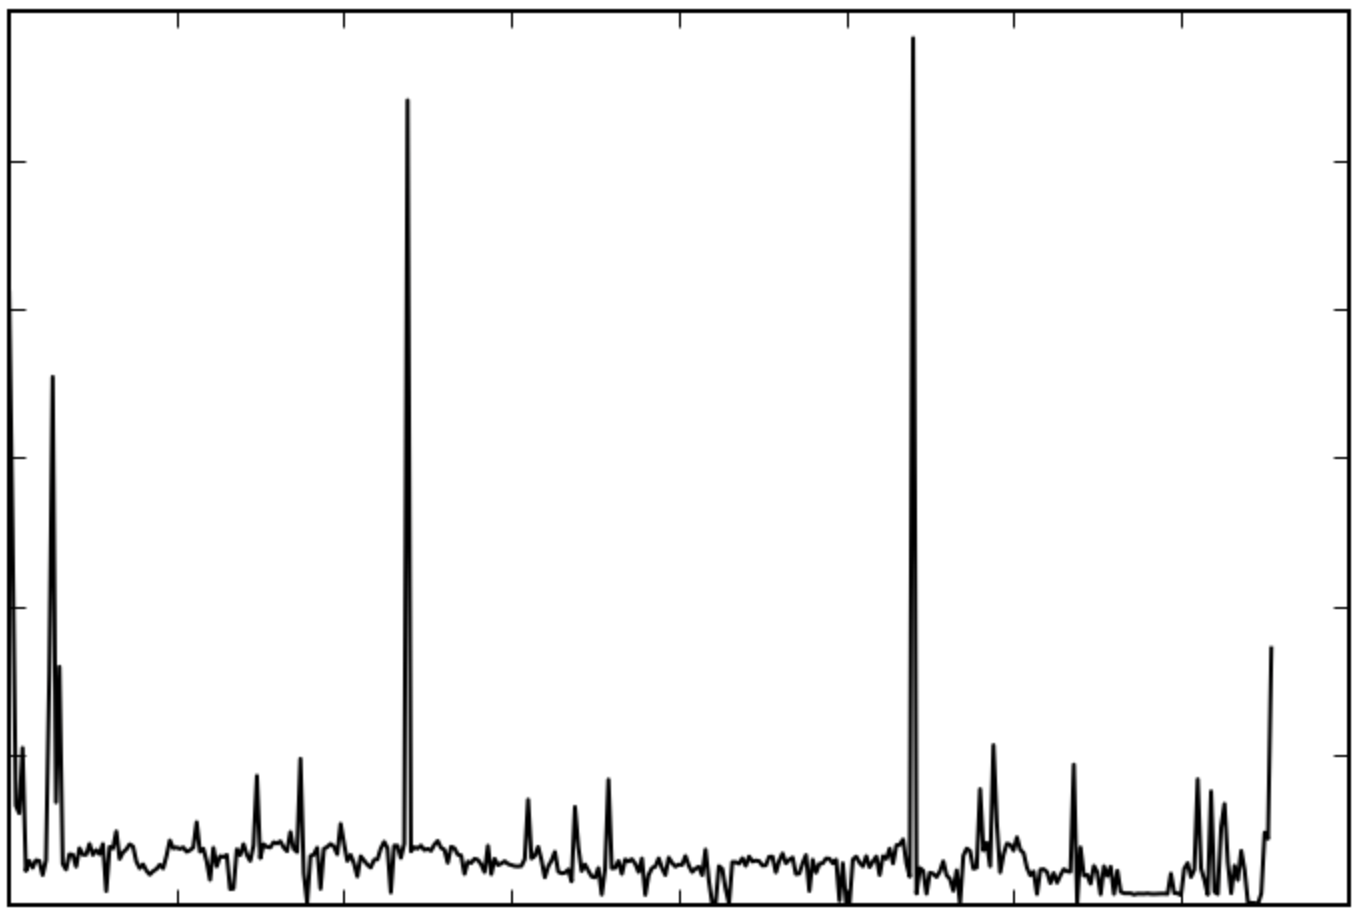
\includegraphics[scale=0.25]{pasted-image-33.png}
        \caption{}
    \end{subfigure}
    \caption{Графики операций (a) QueryBasicInformationFile и (б) ReadFile}
    \label{fig_parsetree}
\end{figure}

Итак мы разделили общий поток операций на несколько и, если в предыдущем параграфе в качестве признака объекта использовалась частота определённой N-граммы, то сейчас мы имеем набор графиков в качестве множества признаков. В отличии от действительных чисел, новые признаки в виде графиков не подходят для прямого использования в линейной модели и нам необходимо использовать другие методы машинного обучения. В данном случае, для решения задачи классификации, мы введём функцию расстояния между двумя сигналами и далее воспользуемся метрическим алгоритмом K ближайших соседей. Данную функцию мы будем использовать для каждого типа графиков в отдельности, поэтому при таком решении у нас возникнет вектор расстояний. Как мы увидим в дальнейшем, используя данный вектор, мы создадим целый набор классификаторов, после чего решим проблему их объединения.

\section{Функция расстояния между сигналами, алгоритм DTW}